\documentclass[11pt]{article}
%\usepackage{graphicx}
%\usepackage{verbatim}
\usepackage{mathtools}
\usepackage{enumitem}
\usepackage{amsfonts}
\usepackage{subcaption}
\usepackage{url}
\usepackage{inconsolata}
\usepackage{ifpdf,graphicx}
\usepackage[shellescape,latex]{gmp}
\usepackage[hmargin=3cm,vmargin=2cm]{geometry}
\ifpdf
  \DeclareGraphicsRule{*}{mps}{*}{}
\fi

\title{Digital Media Coursework: Making a Game}
\author{Matt Thompson, Module code: CM40198}
\begin{document}
\maketitle
\clearpage
\tableofcontents
\clearpage

% Plan:
% - introduce the game idea
% - tech used: Love2d, Lua, Blender, Gimp
% - state machine
% - class descriptions
% - UML class diagram?
% - chroma key process
% - sprite sheets (explain problems with texture size)

\section{Introduction}
This report describes the techniques used to develop a simple ``beat-em-up''-style game that runs on Linux, Mac OSX and Windows.

In this game, two characters compete in a fight where they can punch or kick each other to reduce their opponent's health. They can also perform evasive manoeuvres by crouching and jumping.

Instead of drawing or modelling the characters to put in the game, I used live-action footage of some of my friends punching, jumping, etc in real life. I filmed their actions in front of a green screen, which was then later replaced with the game background using a chroma-keying technique described in section \ref{sec:chroma}. This video footage was then converted into sprite sheets to use as animations in the game (see section \ref{sec:sprites}).

\section{Tools used to make the game}
In order to save time, I opted not to build the game from scratch using a low-level language like C$^{++}$. I instead used a minimalistic game framework, L\"{O}VE2D \cite{love2d}, to handle the low-level OpenGL routines.

\subsection{Game framework and scripting language}
\subsubsection{L\"{O}VE2D} 
L\"{O}VE2D \cite{love2d} is a 2D game creation framework written in C$^{++}$ that allows game programming using the Lua \cite{lua} scripting language. It is released under the zlib license \cite{zlib}, a free and permissive license.

The design of L\"{O}VE2D is very simple. It provides three main callback functions: \texttt{love.load()}, \texttt{love.update(dt)} and \texttt{love.draw()}. There are also callbacks for keyboard events that are called whenever a key is pressed.

The \texttt{love.load()} callback is called when the game loads for the first time. It is only called once, so it is used for initial setup of the game. This can be for things like setting the size of the game window, reading in the animation sprite sheets, and initialising the game objects.

The \texttt{love.update(dt)} callback is called continuously. The `dt' parameter stands for `delta time', and is the amount of seconds since the last time the function was called (which is usually a small value like 0.025). Most of the game logic happens inside this loop.

The \texttt{love.draw()} callback continously draws images to the screen. Functions such as \texttt{love.graphics.draw()} must be called from inside this function in order to change what is displayed on the screen.

\subsubsection{Lua}
L\"{O}VE uses the Lua \cite{lua} scripting language for the programming of game logic. Lua is an `extension programming language', meaning that it only works embedded in a host client. It is an ideal scripting language for games, as its minimalistic featureset allows for extremely fast execution.

Lua is a dynamically typed language that offers good support for object-oriented, functional and data-driven programming paradigms. Interestingly, the only data structure provided out-of-the-box is a table, but the nature of Lua facilitates the extension of these tables into more complex data structures.

Another interesting feature of Lua is its use of \emph{metatables}, which define the behaviour of values under certain special operations. These metatables allow the extension of Lua to create things like instantiatable classes out of tables.

\subsection{Image manipulation tools}
I tried to use only free and open source software to make this game. For this reason, I chose to use Blender \cite{blender}, a 3D modelling tool, for compositing tasks like chroma keying. I used the GIMP \cite{gimp}, an image editor, to stitch together the images produced by Blender into sprite sheets.

Although Blender is traditionally used for 3D modelling and animation, it also has a very sophisticated node editor for compositing work. In section \ref{sec:chroma}, I describe how I used this node editor to remove the green screen from the background of the video footage.

I used a script made by a GIMP user for the creation of sprite sheets to stitch together my animation images \cite{gimpscript}. More details are found in section \ref{sec:sprites}.

\section{Game design}
\begin{figure}[tp]
\centering
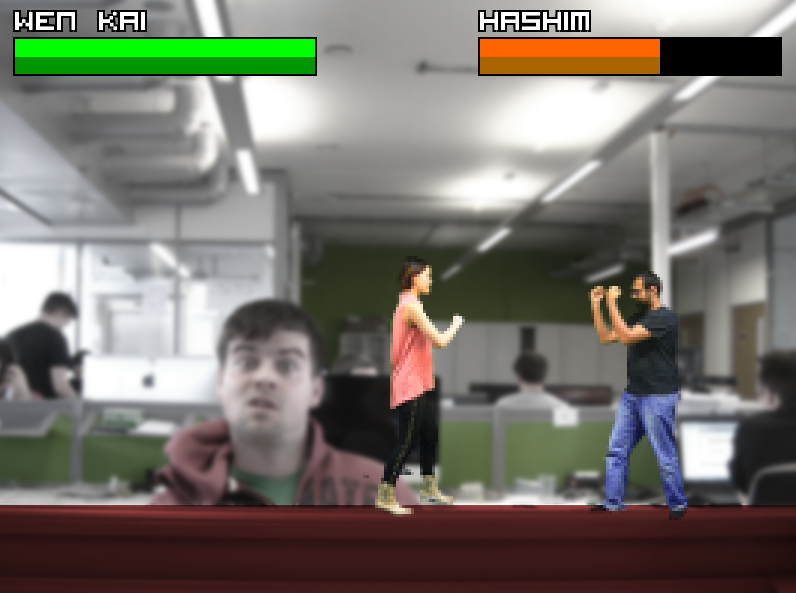
\includegraphics[width=0.8\textwidth]{screenshot.png}
\caption{A screenshot of the gameplay}
\label{fig:screenshot}
\end{figure}

This game is designed to be played by two players. When the game first starts, the players are presented with a character selection screen. Once both players have selected their characters, the game begins.

Player 1's health is represented by a bar in the top left corner of the screen. Player 2 has a bar at the top right. At the bottom of the screen, the player characters themselves appear. 

The players can move towards and away from each other and try to punch and kick. If a player tries to attack the other player and they are close enough, the other player loses some health points, and their health bar shortens. Once a player has lost all of their health points, they `die', and the other player is declared the victor. Figure \ref{fig:screenshot} shows the game in action.

\paragraph{Controls}
Player 1 can move his character around by using the W, A, S, and D keys on the keyboard to jump, walk left, crouch and walk right respectively. The left shift key on the keyboard makes the character punch, the left control key makes them kick.

Player 2 moves his character with the arrow keys, and uses the right shift and right control keys to punch and kick.

Joypad support is partially implemented, however no Linux-compatible joypads could be found for testing.

\subsection{Code structure}
The code is split into seven files: \texttt{main.lua, player.lua, gfx.lua, fight.lua, game.lua, hud.lua} and \texttt{anim8.lua}
\begin{itemize}[noitemsep]
    \item \texttt{main.lua} contains the main L\"{O}VE callbacks (load, update, draw).
    \item \texttt{player.lua} contains the Player class.
    \item \texttt{gfx.lua} contains functions to load animations from image files.
    \item \texttt{fight.lua} contains the Fight class, which manages the interactions between Player objects.
    \item \texttt{game.lua} contains the Game class, which handles the entire game and displays the character selection menu
    \item \texttt{hud.lua} contains the StatusBar and Messages classes, which display the players' health bars and shows text on screen.
    \item \texttt{anim8.lua} is a third-party library for the handling of animations.
\end{itemize}

\subsection{Class descriptions}
\begin{figure}[tp]
    \centering
    \begin{mpost}[mpsettings=input metauml;]
    Class.A("Player")
    ("+name:string","+number:int","+x:int","+y:int","+anims:animation[]","+keymap:string[]","+direction:string","+status:string","+anim:string","+sizex:int","+sizey:int","+health:int","+lock:boolean","+timer:int")
    ("+new(name:string, anims:animation[], keymap:string[]):void","+getHit(height:int,attack:string):void","+takeDamage(amount:int):void","+keyevent(key:string):boolean","+animate(action:string):void","+resetAnim(action:string):void","+render():void","+move(x:int, y:int):void","+flip():void","+die():void","+celebrate():void","+update(dt:float):void","+keyreleased(key:string,unicode:string):void");

    Class.B("Fight")
    ("+player1:Player","+player2:Player","+messages:Message[]")
    ("+new(player1:Player, player2:Player, messages(Message[])):void","+applyDamage():void", "+victory(winplayer:Player):void", "+update(dt:float):void");

    Class.C("StatusBar")
    ("+player:Player","+value:int","+font:Font")
    ("+new(player:Player):void","+draw():void");

    Class.D("Messages")
    ("+message:string","+size:int","+color:int[]","+font:Font","+x:int","+y:int")
    ("+new():void","+announceWinner(winner:string)","+show():void");
    
    Class.E("Game")
    ("+background:Image", "+menuoptions:Player[]", "+players:Player[]", "+statusBars:StatusBar[]", "+keymap:Keymap[]", "+fight:Fight", "+font:Font", "+fighting:boolean", "+menuSelected:int[]")
    ("+new(keymaps:Keymap[],allPlayers:Player[]):void","+keypressed(key:string):void","+startFight():void","+showMenu():void","+update(dt:float):void","+draw():void");

    topToBottom(10)(C, D);
    topToBottom(10)(D, E);
    topToBottom(10)(B, A);
    leftToRight(10)(A, D);
    drawObjects(A,B,C,D,E);
    \end{mpost}
\caption{Classes}
\label{fig:classes}
\end{figure}

The classes are shown in the class diagram in figure \ref{fig:classes}. Constructors are indicated by the ``new'' method of each class.
Although Lua is a dynamically typed language, I have included the expected types in the class diagrams. It should also be noted that all class members are public, since Lua does not offer privacy mechanisms.

\subsection{Finite state machine}
\begin{figure}[tp]
\centering
\begin{mpost}[mpsettings=input metauml;]
Begin.b;
State.rest("Rest")();
State.walk("Walk")();
State.punch("Punch")();
State.kick("Kick")();
State.crouch("Crouch")();
State.jump("Jump")();
State.gethit("Get hit")();
State.lose("Lose")();
State.win("Win")();
End.e;

leftToRight(30)(b, rest);
leftToRight(30)(rest, walk);
leftToRight(30)(crouch, lose);
topToBottom(20)(lose, win);
leftToRight(30)(win, e);
topToBottom(20)(walk,punch,kick,crouch,jump);
leftToRight(30)(punch,gethit);

drawObject(b);
drawObjects(rest,walk,punch,kick,crouch,jump,gethit,lose,win);
drawObject(e);

clink(transition)(b,rest);
clink(transition)(rest,walk);
clink(transition)(walk,rest);
clink(transition)(rest,punch);
clink(transition)(punch,rest);
clink(transition)(rest,kick);
clink(transition)(kick,rest);
clink(transition)(rest,crouch);
clink(transition)(crouch,rest);
clink(transition)(rest,jump);
clink(transition)(jump,rest);
clink(transition)(rest,gethit);
clink(transition)(walk,gethit);
clink(transition)(punch,gethit);
clink(transition)(kick,gethit);
clink(transition)(crouch,gethit);
clink(transition)(jump,gethit);
clink(transition)(gethit,rest);
clink(transition)(gethit,lose);
clink(transition)(punch,win);
clink(transition)(kick,win);
clink(transition)(lose,e);
clink(transition)(win,e);

\end{mpost}
\caption{Player state machine}
\label{fig:stateDiagram}
\end{figure}

The game is a very simple finite state machine with nine different states:
\begin{itemize}[noitemsep]
    \item Rest
    \item Walk
    \item Punch
    \item Kick
    \item Jump
    \item Crouch
    \item Get hit
    \item Win
    \item Lose
\end{itemize}

Each player starts off in a `rest' state. Pressing the left or right keys transitions them into a `walk' state. Pressing up goes into the `jump' state, and holding the down key makes the player crouch. The player returns to the rest state once the down key is released. Punch and kick states are entered when their respective keys are pressed, returning to the rest state once their animations have played once through.

When a player gets punched or kicked by the other player, they enter their `get hit' state, which plays an animation for a while before returning to the resting state.

It should be noted that each state corresponds to an animation. While an animation is playing, the player remains in that state.

If a player has been hit many times by the other player and their health value reaches zero, they go into the `lose' state, from which there is no return. The other player ends in the `win' state.

A diagram of the player state machine is shown in figure \ref{fig:stateDiagram}.

\section{Animation techniques}
\subsection{Chroma keying}\label{sec:chroma}
\begin{figure}[tp]
\centering
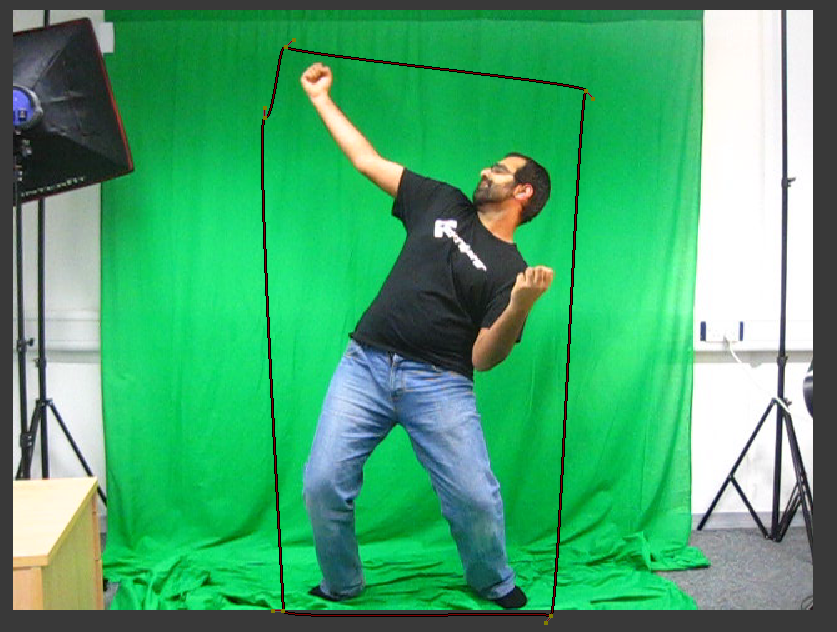
\includegraphics[width=0.6\textwidth]{mask.png}
\caption{A frame from the captured video footage. A mask has been drawn around the desired area.}
\label{fig:mask}
\end{figure}

Chroma key compositing is a technique for layering two images together. One image, the `foreground image' has a mask of transparent pixels (alpha mask) applied according to a set of colour hues (chroma range). This technique is also commonly referred to as green screen or blue screen, since these are the colours typically chosen to be replaced with alpha pixels.

Typically, a function like this is applied to every pixel in an image:

$$f(r, g, b) \rightarrow \alpha$$

If the function returns $\alpha \leq 0$, this means the pixel is in the green screen area and will become transparent. If $\alpha \geq 1$, then the pixel will be part of the foreground. If $0 < \alpha < 1$, then the pixel will be partially transparent, with some of the foreground still visible.

In this implementation, I also used Blender's node editor to do screen spill removal. A simple example of such a function, again applied to all pixels in the image, would be:

$$g(r, g, b) \rightarrow (r, \min(g, b), b)$$

This function removes any kind of coloured `tinge' that may exist around the edges of the foreground image after chroma keying is applied.

Figure \ref{fig:mask} shows a frame from the video footage for an animation. A mask has been drawn around the area of interest to be chroma keyed. Figure \ref{fig:compositing} shows how the image looks in Blender's node editor once the chroma key and color spill functions have been applied.

\begin{figure}[tp]
\centering
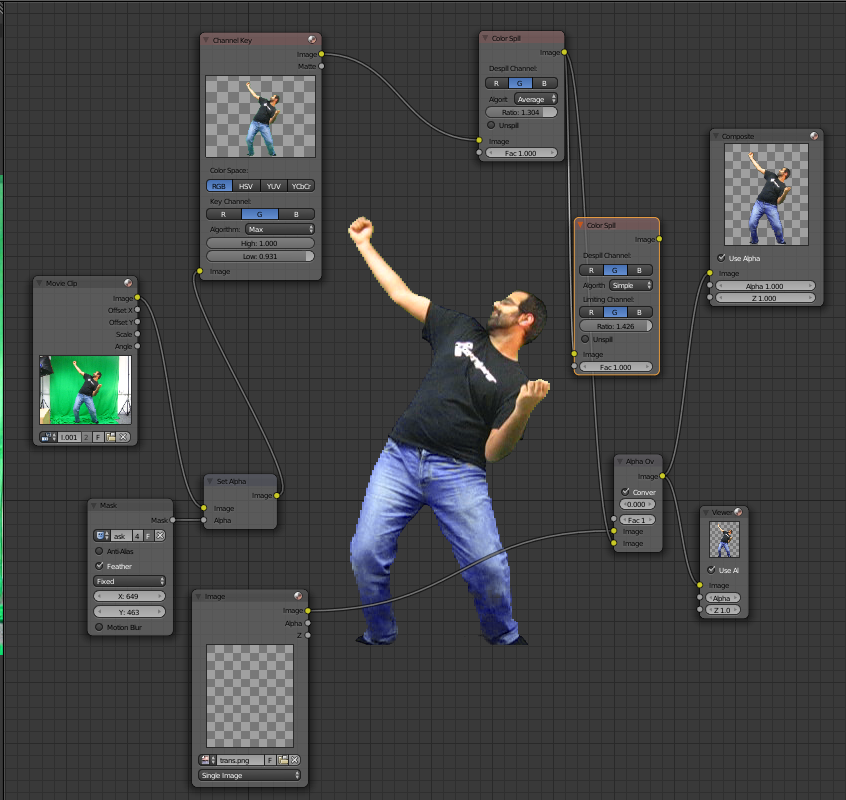
\includegraphics[width=0.8\textwidth]{blender.png}
\caption{Blender's compositing node editor}
\label{fig:compositing}
\end{figure}

\subsection{Sprite sheets}\label{sec:sprites}
\begin{figure}[tp]
\centering

\includegraphics[width=1.0\textwidth]{win.png}
\caption{The final sprite sheet for Hashim's ``winning'' animation}
\label{fig:win}
\end{figure}
In the game, each character is represented by a sprite, which is simply a 2D image with a transparent background. Each action for each character has a set of images which make up its animation sprite.

While it would be perfectly possible to store every image for an animation separately, this is often inconvenient. I decided to use sprite sheets to use one file per animation.

A sprite sheet contains many images arranged together in a grid. Each row in the grid represents a separate animation, with each column of the row being one frame of the animation.

Initially, I wanted to store all the animations for each character in a single sprite sheet, with one row per animation. However, this resulted in a final image that was much too large to handle. Since each player sprite is 100 pixels tall by 100 pixels wide, the total dimensions of the image soon exceeded 2048 by 2048, which is the maximum texture size for most graphics cards. Since L\"{O}VE2D stores sprite sheets as OpenGL textures, a sprite sheet that exceeded this maximum size would just be displayed as a white box.

For this reason, I instead used one sprite sheet per character animation. Figure \ref{fig:win} shows the sprite sheet for one character's ``winning'' animation.

\section{Evaluation and future work}
AI for the game characters will need to be implemented in order to support a single-player game mode. Also, music and sound effects need to be added to make a more immersive game experience. It would also be nice to add more characters and joypad support in the future.

The game has plenty of bugs. For example:

\begin{itemize}[noitemsep]
    \item Selecting the same character for both players results in only one character appearing on the screen, who then beats themselves up.
    \item Pressing a key while a character is jumping makes them get `stuck' in midair.
    \item Players can still inflict damage when attacking in the wrong direction.
    \item Players can still be moved when dead.
    \item The only way to replay the game is to close and re-open it.
\end{itemize}

At the moment, this game is just a proof-of-concept, but I do hope to develop and polish it a little further. The full source code can be found online at \texttt{http://github.com/cblop/bloodbath}.

\bibliographystyle{plain}
\bibliography{report}

\end{document}

